\subsection{Applications}
In this section, we evaluate the performance of the runtime system using benchmarks taken from 3 HPC dwarfs: Sparse Cholesky Factorization (Sparse Linear Algebra), 2.5D Cannon's Matrix Multiplication (Dense Linear Algebra), and 3D Stencil (Structured Grids).
For each application, we develop multiple code variants to evaluate individual components of the runtime on GPUs.

\subsubsection{Sparse Cholesky Factorization}
Sparse Cholesky Factorization A= $LL^T$, where A is a sparse and symmetric positive-definite matrix,
appears in many scientific and engineering problems.
Depending on the sparsity pattern of the input matrix, many sparse representations can be used.
In this paper we employ the CSC (Compressed Sparse Column) format. 
The input matrix is organized as a list of "non-zero" tiles, each including lists of non-zero elements and their row and column indices.
The factorization operation is comprised of 3 smaller kernels: {\em factor}, {\em solve}, and {\em update}.
These computations on CSC tiles and their data dependencies can be represented by a DAG as shown in Fig.~\ref{fig:cholesky}. 
For very sparse matrices, this DAG may consist of many small tasks.
Thus, this is a perfect application to evaluate the benefit of the fine-grained task scheduling support of the runtime.
We place data on the host's DRAM and execute {\em factor} and {\em solve} on the host's worker.
The compute-intensive {\em update} kernel is executed on GPUs workers.
{\em RambutanAcc} automatically streams data required by this kernel to the GPUs DRAM and streams the results back.

\begin{figure}[htb]
\centering
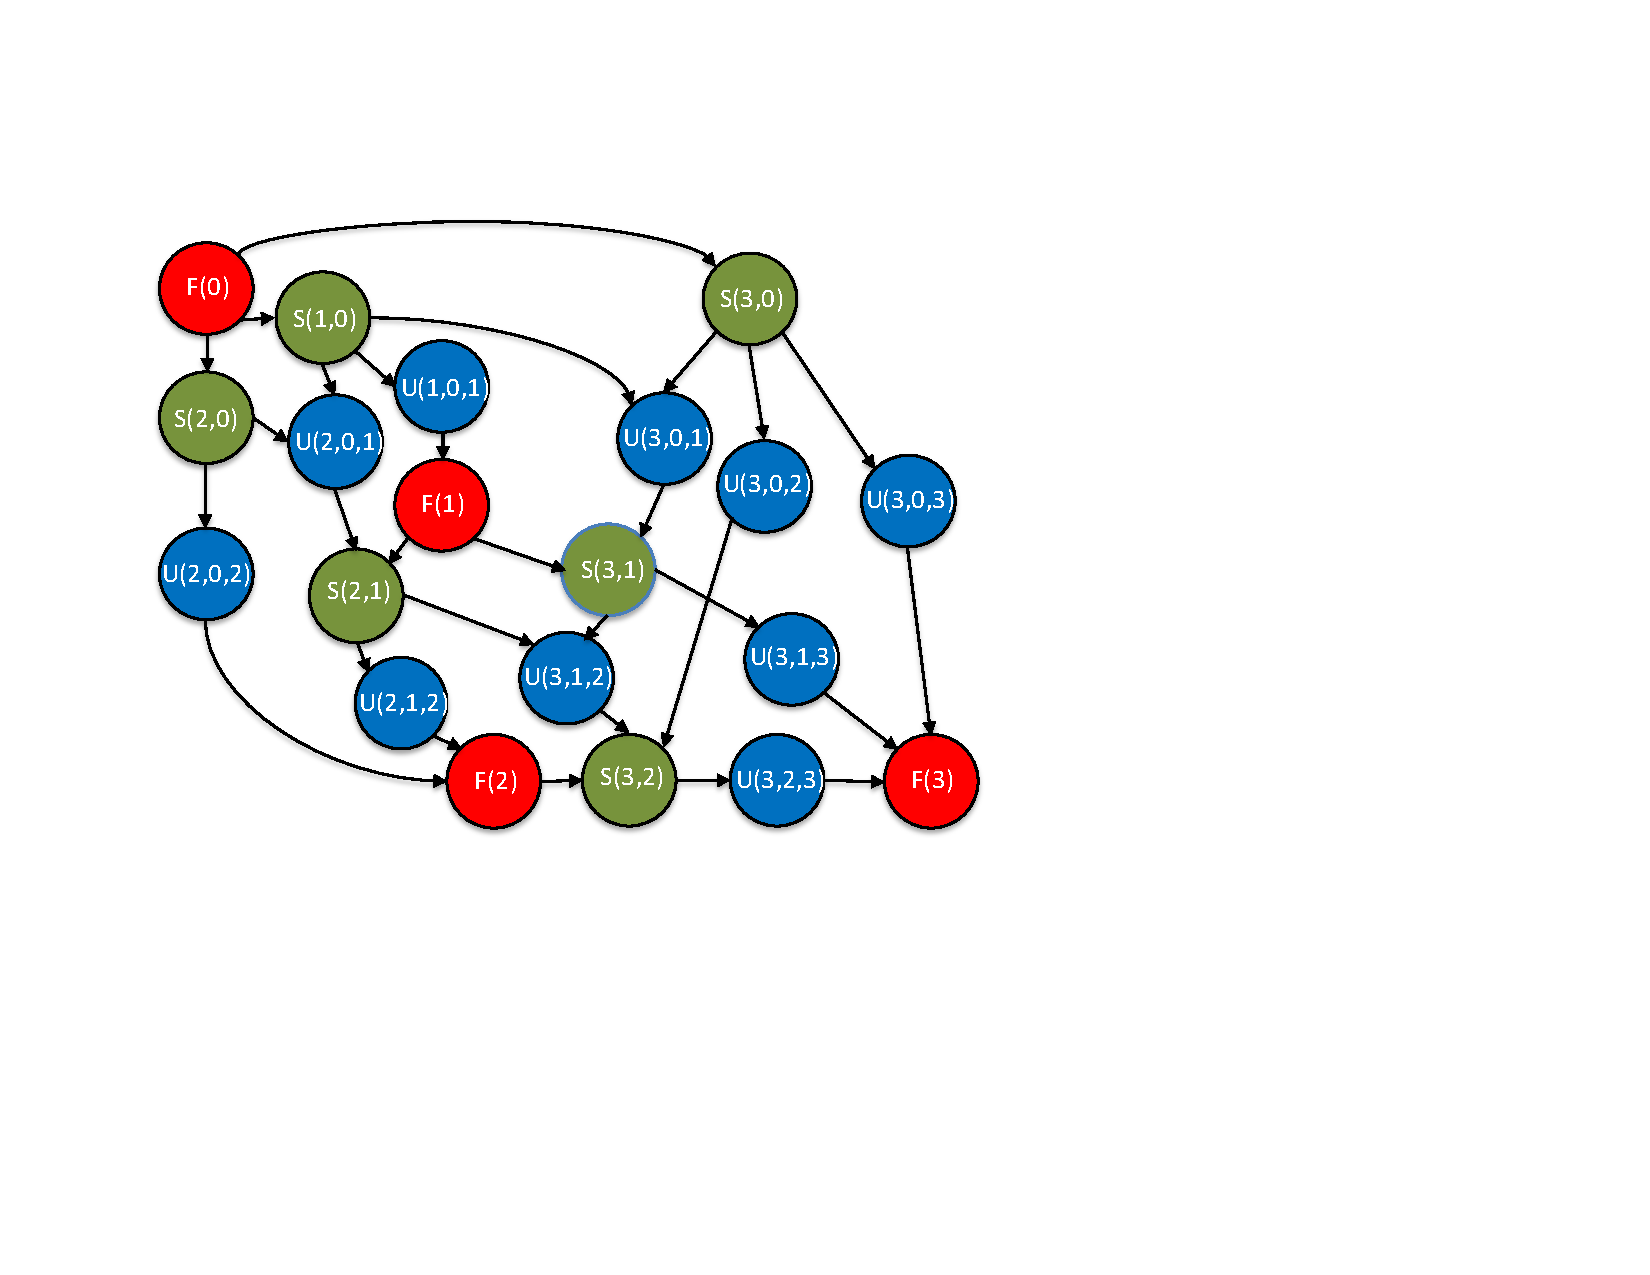
\includegraphics[width=.4\textwidth]{figures/cholesky.pdf}
\caption{Cholesky factorization DAG consisting of 3 types of tasks: F (Factor), S (Solve), U (update). Each task is associated with a partition of the input matrix called {\em tile}. Arrows presesent data dependencies between tasks of different types or of the same task type but on different tiles.}
\label{fig:cholesky}
\end{figure}


\subsubsection{Communication Avoiding Matrix Multiplication}
Although sparse representations are widely used in practice, dense matrix operations also have a significant share in many scientific and engineering areas.
As a result, we employ a dense matrix multiplication operation $C = \alpha* A * B + \beta C$ to evaluate our runtime.
This is a compute bound application, and GPUs architecture is very well suited for the computation. 
There are many algorithms for the matrix multiply operation, and we use a well-known extension of the standard 2D Cannon's algorithm called {\em Communication Avoiding} AKA 2.5D Cannon~\cite{25Dcannon}. 
Under the original 2D Cannon's algorithm, the available tasks are organized into a {\em T=PxP} mesh, partitioning each of the 3 matrices A, B, and C into blocks.
These partitions are first aligned using a skewing operation.
The algorithm then performs P computation steps accumulating the C partition using the rotated A and B partitions.
The communication avoiding algorithm shown in Fig.~\ref{fig:25DCannon} replicates the input matrices by a factor of L using an additional task dimension.
The algorithm broadcasts input data to layers in this dimension to compute the traditional Cannon with T/$\sqrt(L^3)$ steps then reduces the results back to the first layer.


\begin{figure*}[htb]
\centering
\begin{subfigure}[b]{0.4\textwidth}
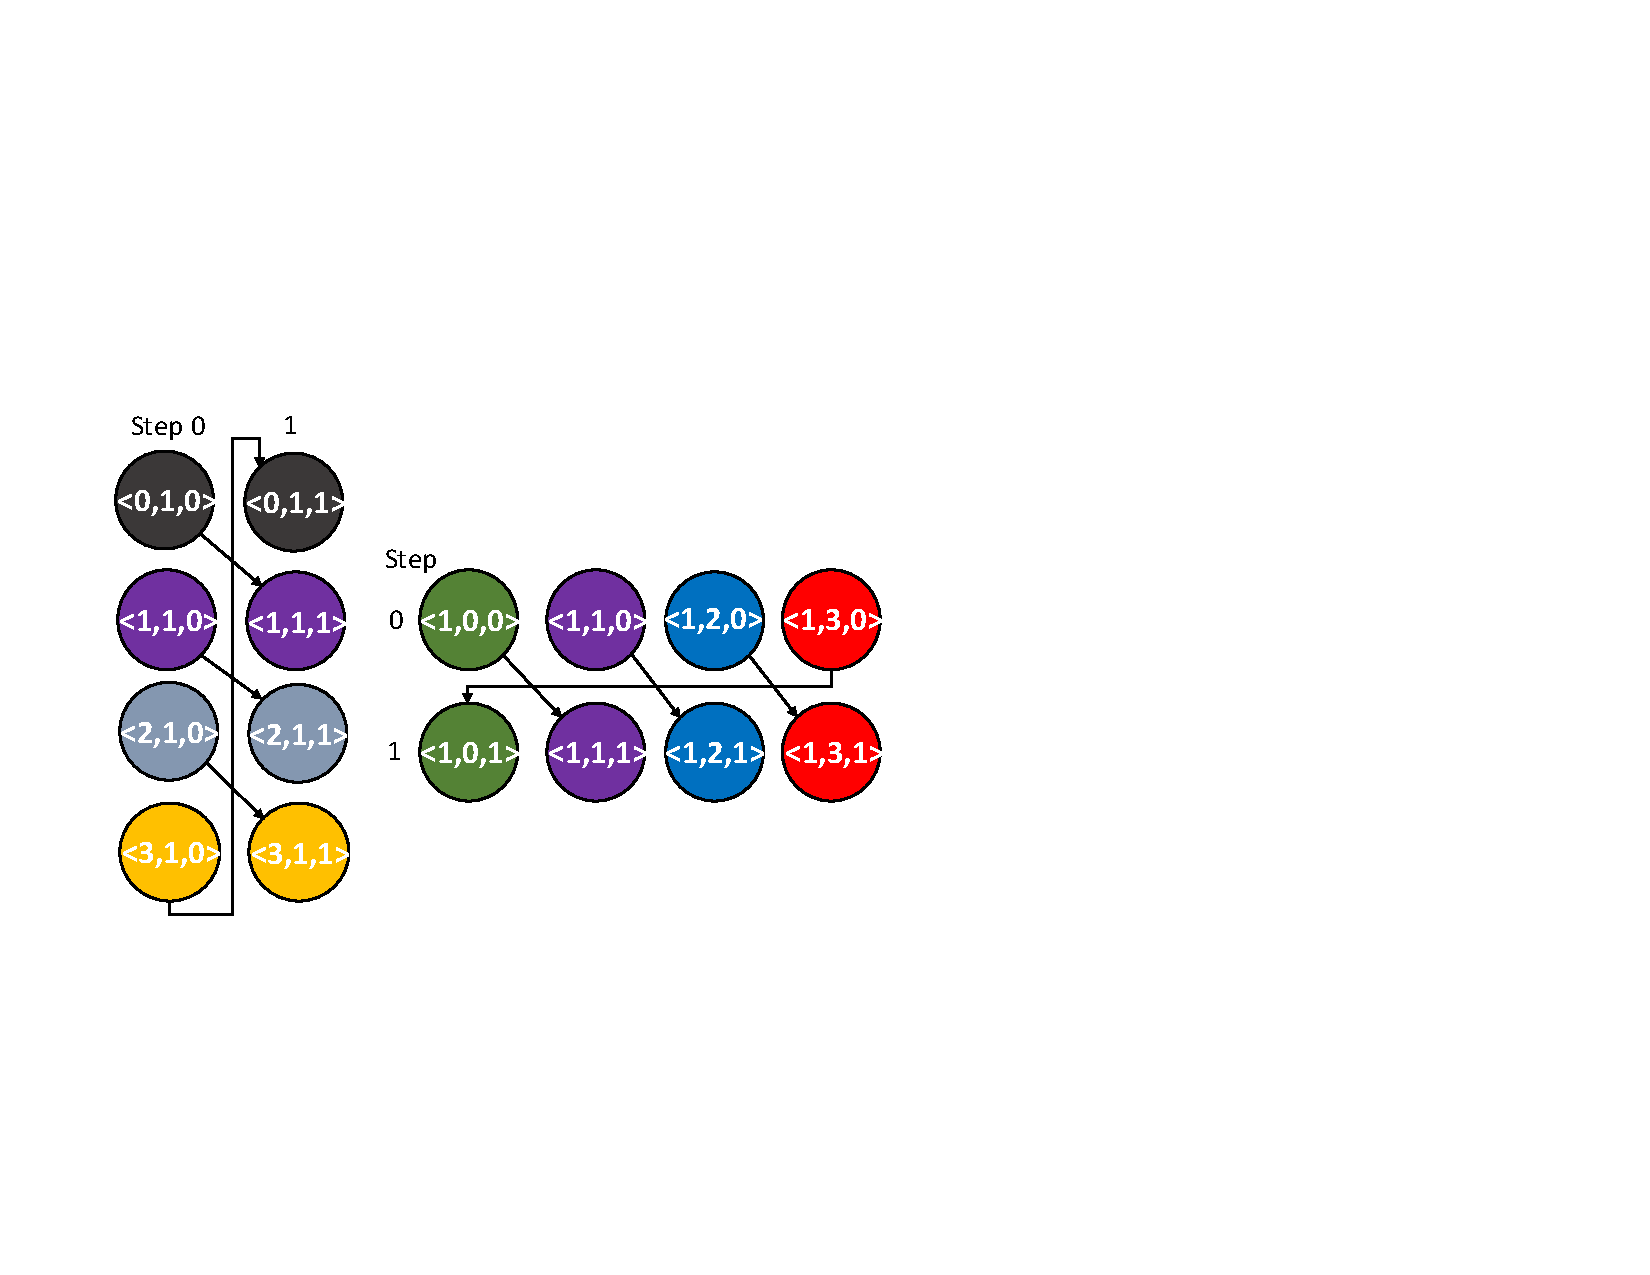
\includegraphics[width=\textwidth]{figures/cannon0.pdf}
\caption{A and B dependencies on each replication layer}
\label{deps}
\end{subfigure}
\begin{subfigure}[b]{0.4\textwidth}
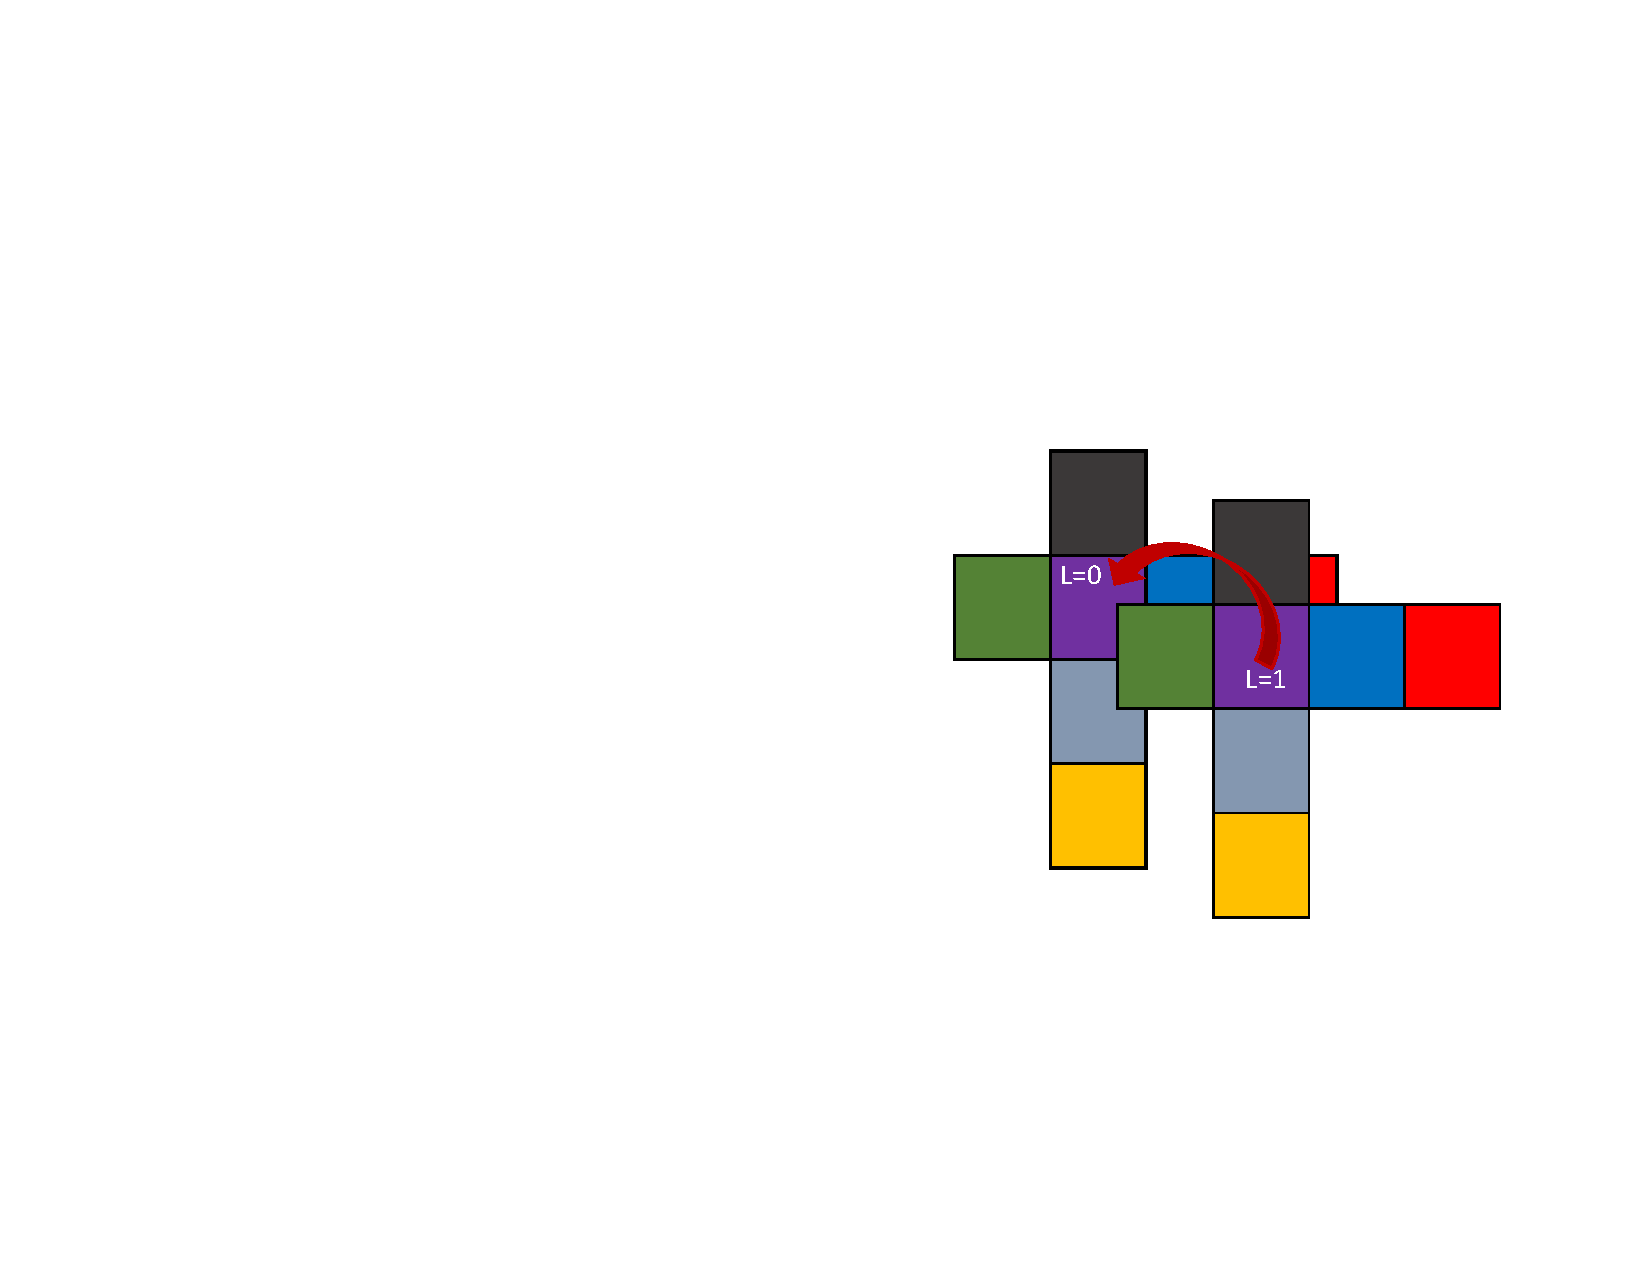
\includegraphics[width=\textwidth]{figures/cannon1.pdf}
\caption{Results are reduced to the original layer}
\label{dataspace}
\end{subfigure}
\caption{Computing $C= \alpha A * B + \beta C$ using the 2.5D Cannon's matrix multiplication algorithm given the input matrices are already replicated and aligned. 
The DAG partitions matrix C and the step space of the algorithm.
Task Id is a triple where the first two numbers represent the coordinates of a C partition and the last is the step number of the algorithm. 
Fig.~\ref{deps} shows 2 subsets of the graph to illustrate 2 types of data dependecies required to compute C.}
\label{fig:25DCannon}
\end{figure*}


\subsubsection{3D Stencil}
The last application is {\em 3D Stencil}, an iterative solver for Laplace's equation in 3 dimensions.
{\em 3D Stencil} iterates over a 3D mesh, updating data elements using values from 6 nearest neighbors.
The DAG for this application is similar to that shown earlier in Fig.~\ref{fig:taskGraph}, except for the number of dimensions.
In particular, each task is associated with a data partition with up to 6 ghost cells.
A task can be run when the previous iteration on this data partition finishes and it pulls all the needed ghost cells from neighboring tasks.
3D stencil is a memory bandwidth bound application. 
Thus using GPUs can boost up the performance significantly.
It is interesting to know if {\em RambutanAcc} can improve the performance further by  hiding communication overheads.


\subsection{System Specifications}
We evaluate the {\em RambutanAcc} runtime on Comet, a GPUs cluster based on Haswell CPU and K80 GPUs and located at the San Diego Supercomputer Center (SDSC).
A K80 GPUs pairs 2 GPUs cards each having 2496 CUDA cores organized into 13 SMs.
The whole K80 GPUs is equipped with 24GB DRAM with up to 480 GB/s memory bandwidth.
Compute nodes on Comet are connected via Mellanox FDR Infiniband interconnects.
We use the nvcc compiler version 7.0 and sm\_35 capability for CUDA codes and Intel compiler for codes running on the host.
We use GASNet for communication among GPUs. 


\subsection{CUDA kernels}
When evaluating the fine-grained scheduling support, to have an apples-to-apples comparison we always use our own CUDA kernels for both coarse and fine-grained scheduling policies.
In these kernels, we perform many optimization techniques such as memory coalescing and spatial tiling using shared memory and register.
For other tests, we use both self developed and vendor provided kernels.
In particular, for Sparse Cholesky Factorization, we develop our own CUDA kernels since there is a routine that has not been provided by standard libraries such as cuSPARSE.
That is, $C = \alpha* A * B + \beta C$ where A, B, and C are all in the {\em sparse} form.
For 2.5D Cannon, we use the cuBLAS's {\em dgemm} implementation included in the NVIDIA toolkit to perform local matrix multiplication.
For 3D Stencil, we use a self-developed CUDA kernel to perform Jacobi sweeps.

\subsection{Coarse v.s. fine-grained scheduling on GPUs}
We first tune computational kernels on a single GPUs.
An interesting path to explore is the tradeoff between coarse and fine-grained scheduling policies.  
Here we use two opposite applications to observe the tradeoff.
For sparse cholesky, the matrix is represented by many small CSC tiles.
Thus, even a small problem size can result in many tasks.
2.5D Cannon, however, is based on a coarse decomposition scheme.
As a result, a data tile can be as large as the data partition assigned to a GPUs.
Fig.~\ref{fig:coarseFine} shows results of sparse cholesky and 2.5D Cannon under two scheduling policies.
It can be seen that on sparse cholesky fine-grained scheduling policy outperforms the coarse-grained one.
This can be explained as follows.
Each CSC tile is very small (e.g. 32x32), making it hard to map computations efficiently to many CUDA cores.
Thus, it may not be posible to scale a task to all available SMs of a GPUs.
We observe that for many input matrices tasks run more efficiently after reducing the number of SMs per worker by a factor of 2 or 4.
Since there may have many tasks that can be runnable at a time, the scheduler can keep all SMs busy at very small overhead.
Fig~\ref{fig:nWorkers} shows the optimal number of workers on a K80 GPUs for Sparse Cholesky Factorization when the degree of sparsity of the input matrix varies.
If the sparse matrix is filled with many tasks we have more parallelism, allowing us to configure the GPUs with more workers.

\begin{figure*}[htb]
\centering
\begin{subfigure}{0.29\textwidth}
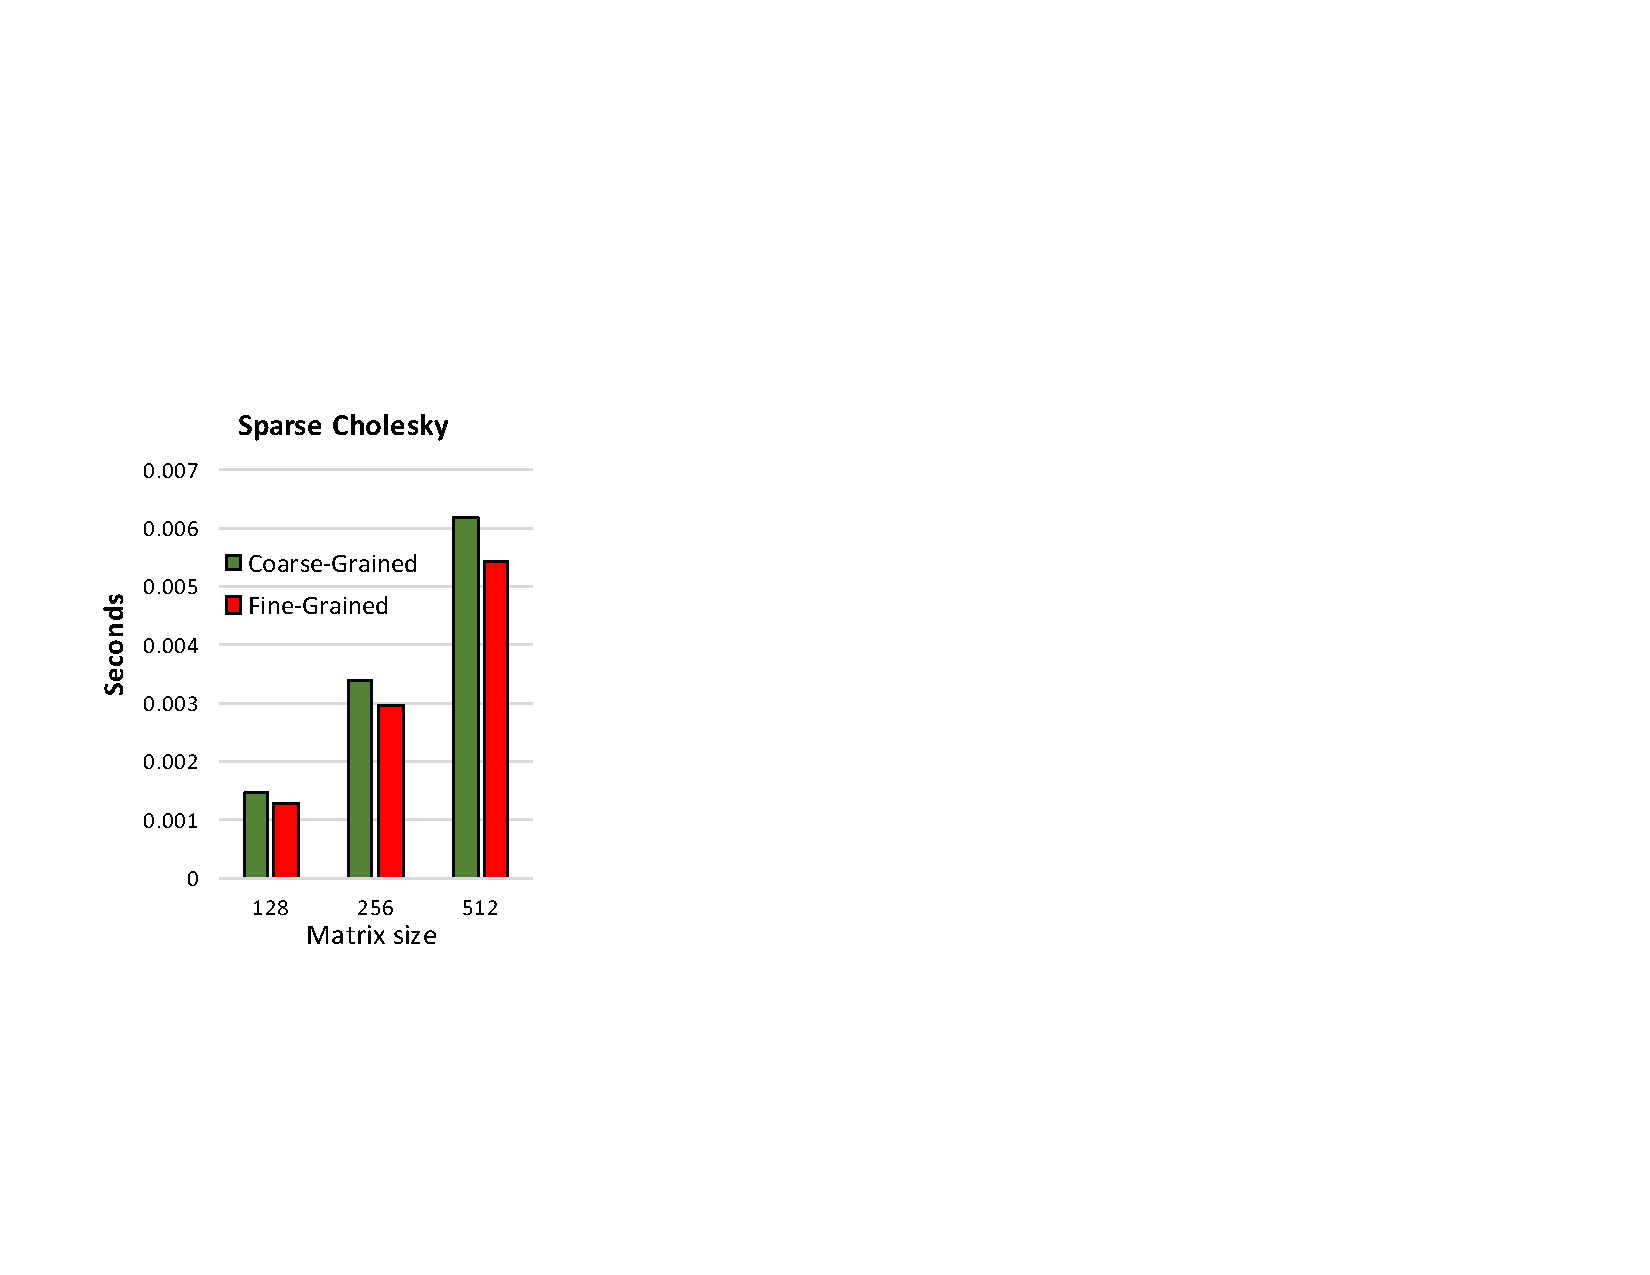
\includegraphics[width=\textwidth]{figures/choleskyScheResults.pdf}
\caption{Tile size 32x32}
\label{choleskySche}
\end{subfigure}
\begin{subfigure}{0.29\textwidth}
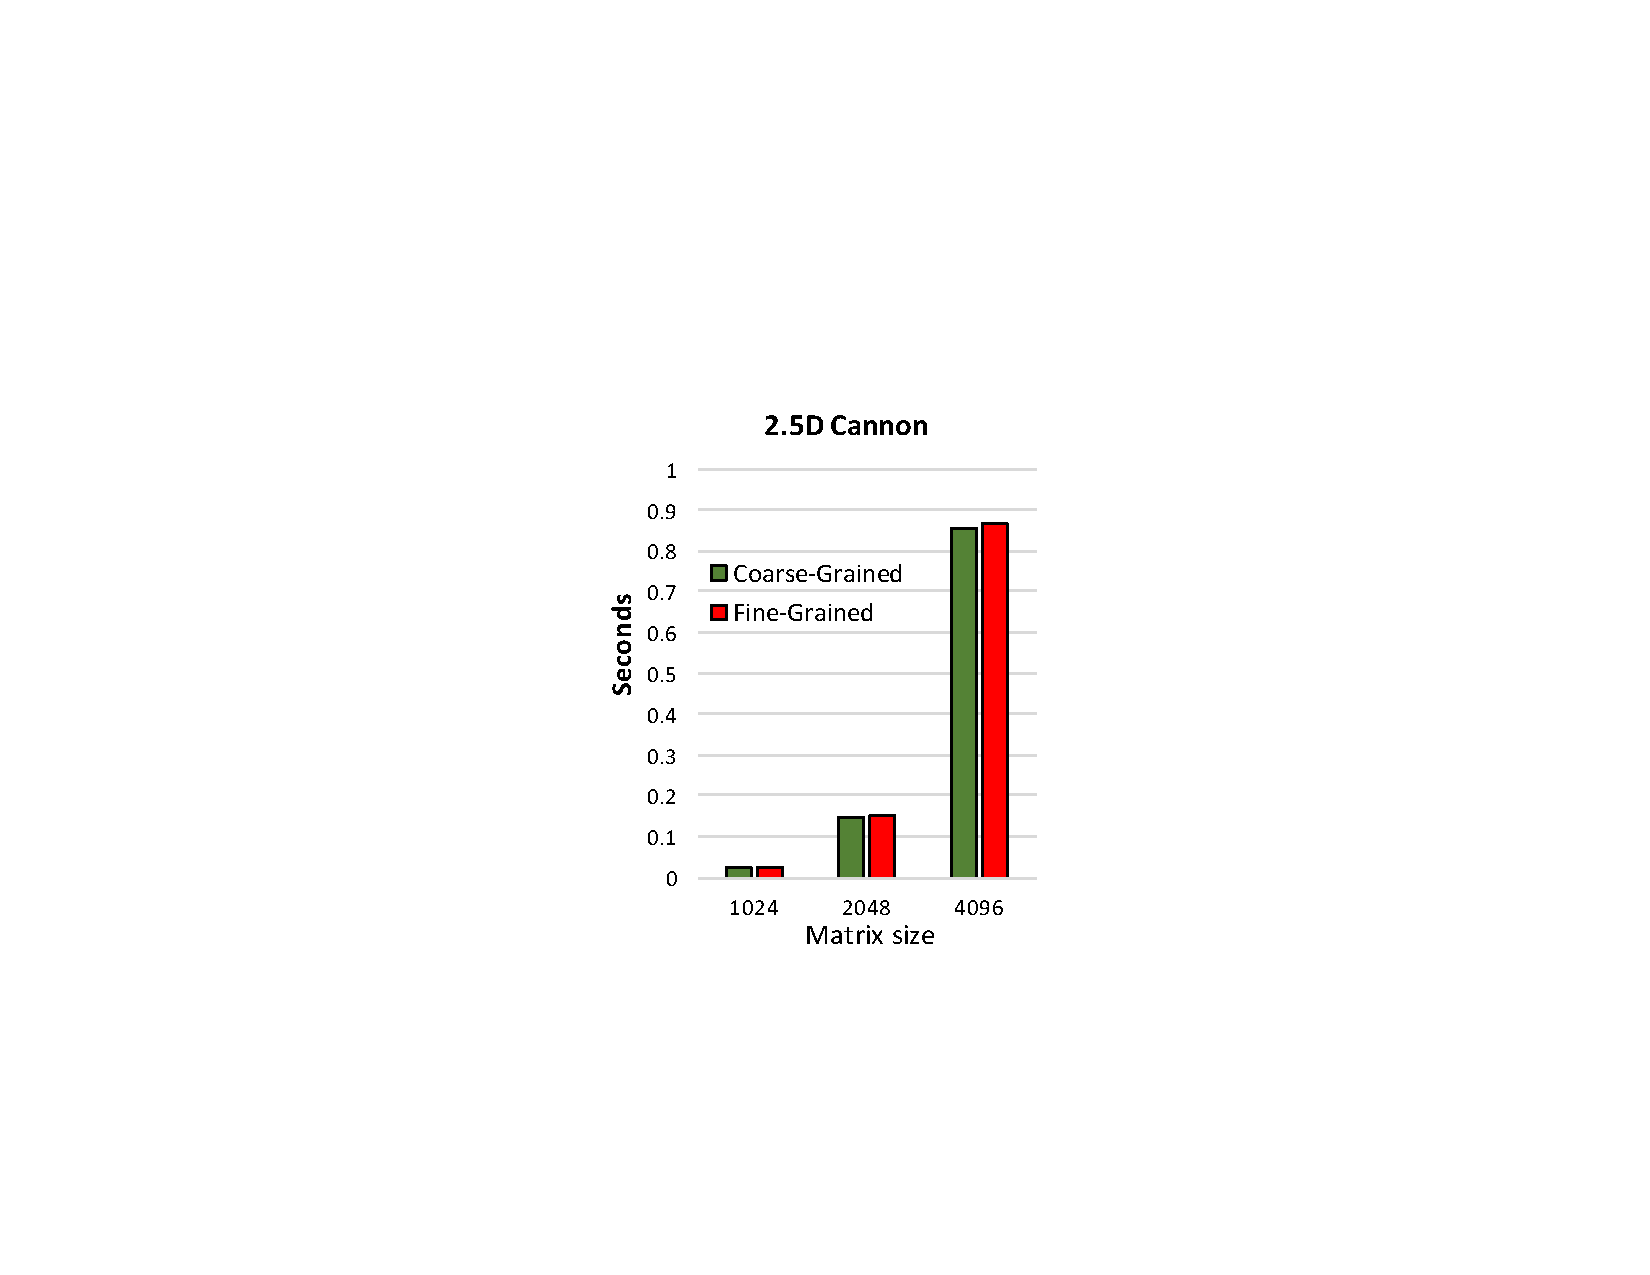
\includegraphics[width=\textwidth]{figures/25DCannonScheResults.pdf}
\caption{Tile size = problem size}
\label{CannonSche}
\end{subfigure}
\begin{subfigure}{0.33\textwidth}
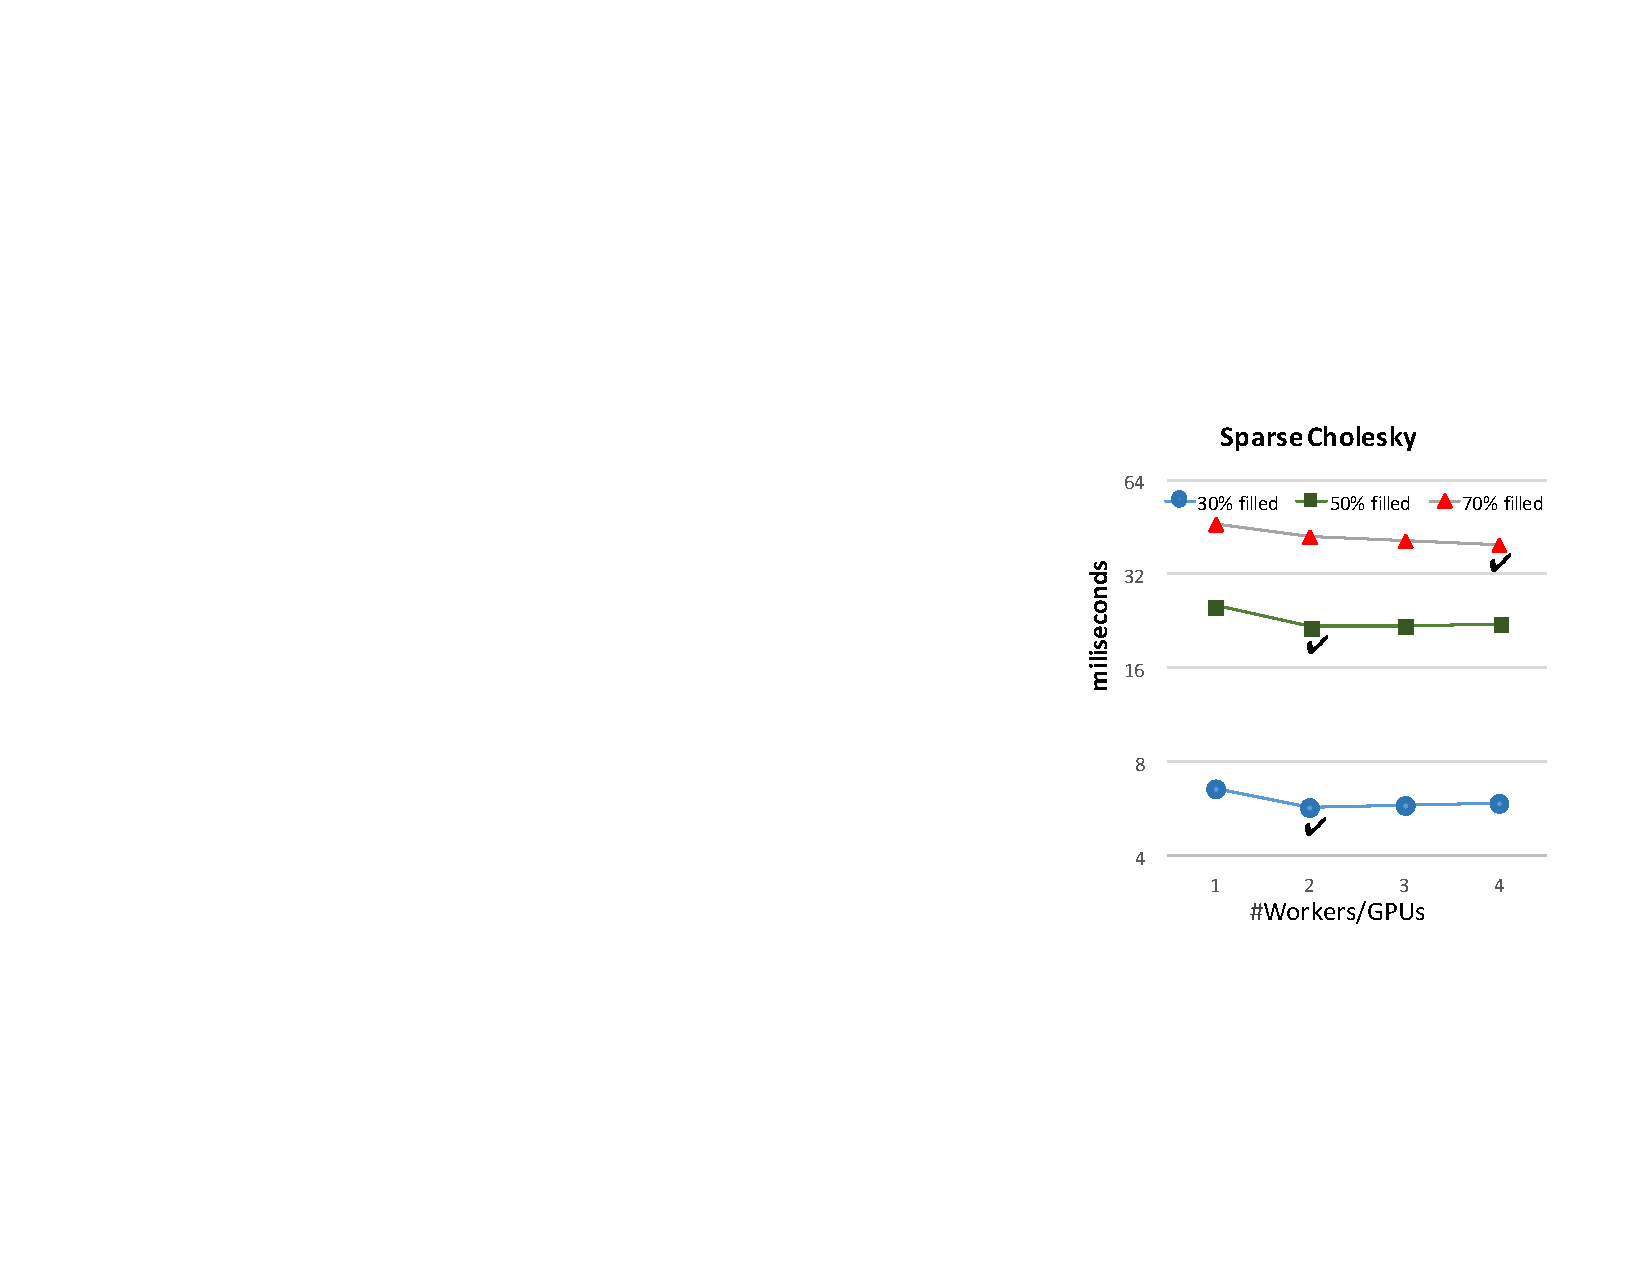
\includegraphics[width=\textwidth]{figures/nWorkers.pdf}
\caption{The optimal number of workers/GPUs}
\label{fig:nWorkers}
\end{subfigure}
\caption{Coarse v.s. fine-grained Scheduling}
\label{fig:coarseFine}
\end{figure*}





Unlike sparse cholesky, we do not see any performance benefit of fine-grained scheduling policy on 2.5D Cannon.
Coarse grained policy even performs slightly better than fine-grained policy.
This result is fairly easy to explain.
Indeed, each 2.5D Cannon task performs many floating point operations due to large and dense data partitions.
The result is that the CUDA kernel can be scaled to all available SMs of a GPUs without significant degradation in efficiency.
The fine-grained scheduling policy requires many tasks to keep all SMs busy.
Thus, we have to over-decompose tasks to obtain more parallelism.
Unfortunately, over-decomposition incurs some overhead as we can see in Fig.~\ref{CannonSche}.
We observe similar results with 3D Stencil.

The lesson learn from this study is that fine-grained scheduling can be very helpful if we have a DAG with many small tasks, which can not run well on the whole GPUs.
This is an important observation since sparse representation is very common in practice.
{\em RambutanAcc} runtime supports fine-grained task scheduling, a simple yet powerful solution to this problem.
The programmer can obtain high compute throughput on GPUs without complicating the application algorithm.

\begin{figure}[htb]
\centering
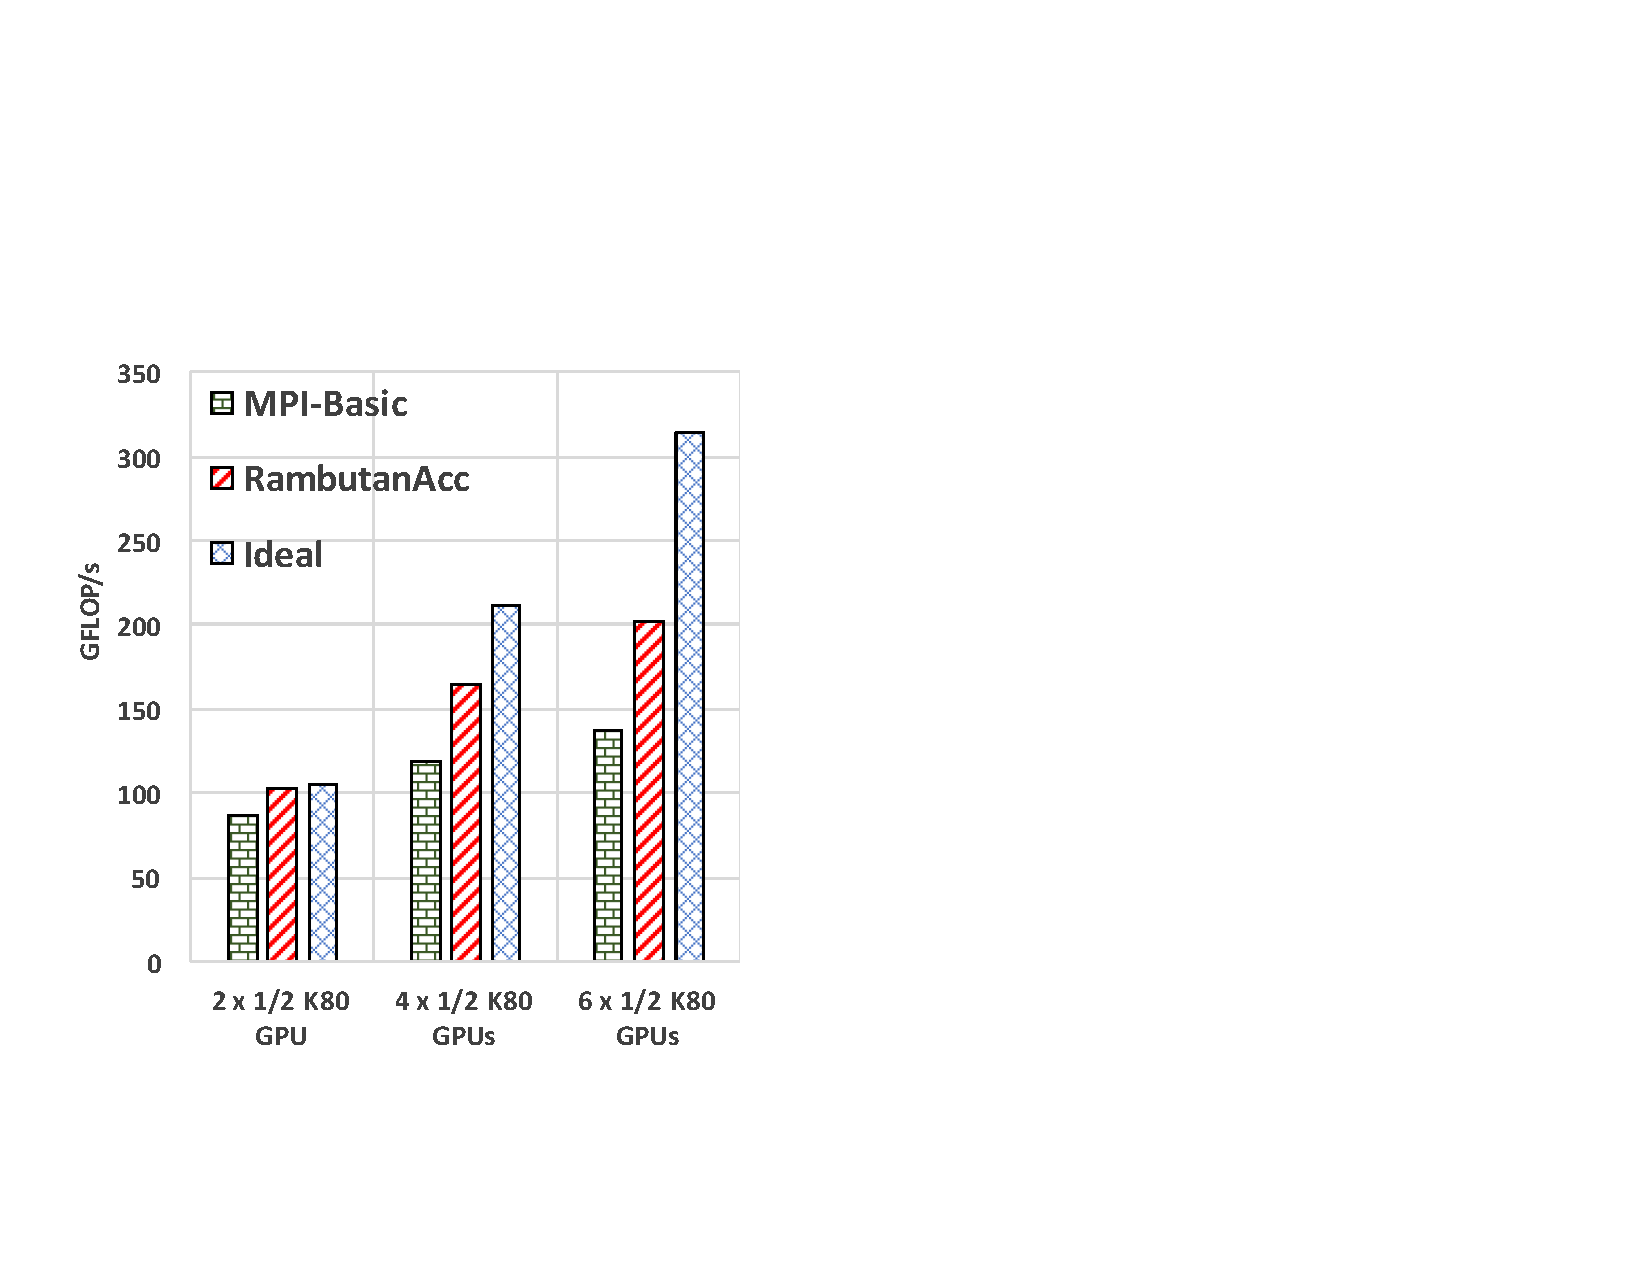
\includegraphics[width=0.49\textwidth]{figures/stencil_tida.pdf}
\caption{Weak scaling study on a single compute node consisting of 2 K80s (4 GPUs)}
\label{stencil_onnode}
\end{figure}


\subsection{Communication hiding}
We now extend the experiment to multiple GPUs.
In this experiment, we evaluate the benefit of hiding the communication overheads among GPUs.
To this end, we configure the runtime in two modes: {\em no overlap} and {\em overlap}.
The former uses blocking CUDA memory copy routines to transfer data between host and GPUs while the latter uses non-blocking variants.
Since the fine-grained scheduler is not compatible with blocking mode (the persistent kernel runs to completion while blocking routines can't proceed until all previously submitted CUDA kernels have completed), we use the coarse-grained scheduling policy for both the blocking and non-blocking modes.

Fig.~\ref{overlap} shows results of 3 applications under two communication modes.
In this study, we do not replicate the input matrices of the 2.5D Cannon's algorithm because the communication avoiding technique may interfere with the communication overlap.
We will study this interference later in Sec~\ref{subsec:CAvsOlap}.
It can be seen in Fig.~\ref{overlap} that on 3 applications {\em overlap} always outperforms {\em no overlap}.
In Cholesky, we place data on the host and stream them to GPUs to perform the compute-intensive {\em update} kernel.
Thus, even on 1 GPUs communication arises.
\footnote{Although we do not show results of 2.5D Cannon and 3D Stencil on 1 GPUs, it's worth noting that computing on 1 GPUs doesn't incur communication cost since we initially place data on GPUs.
As a result, we do not observe performance improvement when running these 2 applications on 1 GPUs.}
On multiple GPUs, we realize notable performance improvement via overlapping communcation with computation.
The overall time reduction is 10\% more or less.
For Stencil, however, we see a higher speedup (up to 1.85x) due to the following reason.
At a small scale 1D decomposition works best since it does not require the costly packing and unpacking operations.
However, with a 1D decomposition scheme the amount of communication does not decrease as the number of GPUs increases.
Thus, the more GPUs the higher communication relative to computation, resulting in a better improvement due to overlap.
Unlike 3D Stencil, experiments on the other 2 applications use a 2D decomposition scheme.
Thus, the communication over computation ratio does not change much as the number of GPU increases.

\begin{figure*}[htb]
\centering
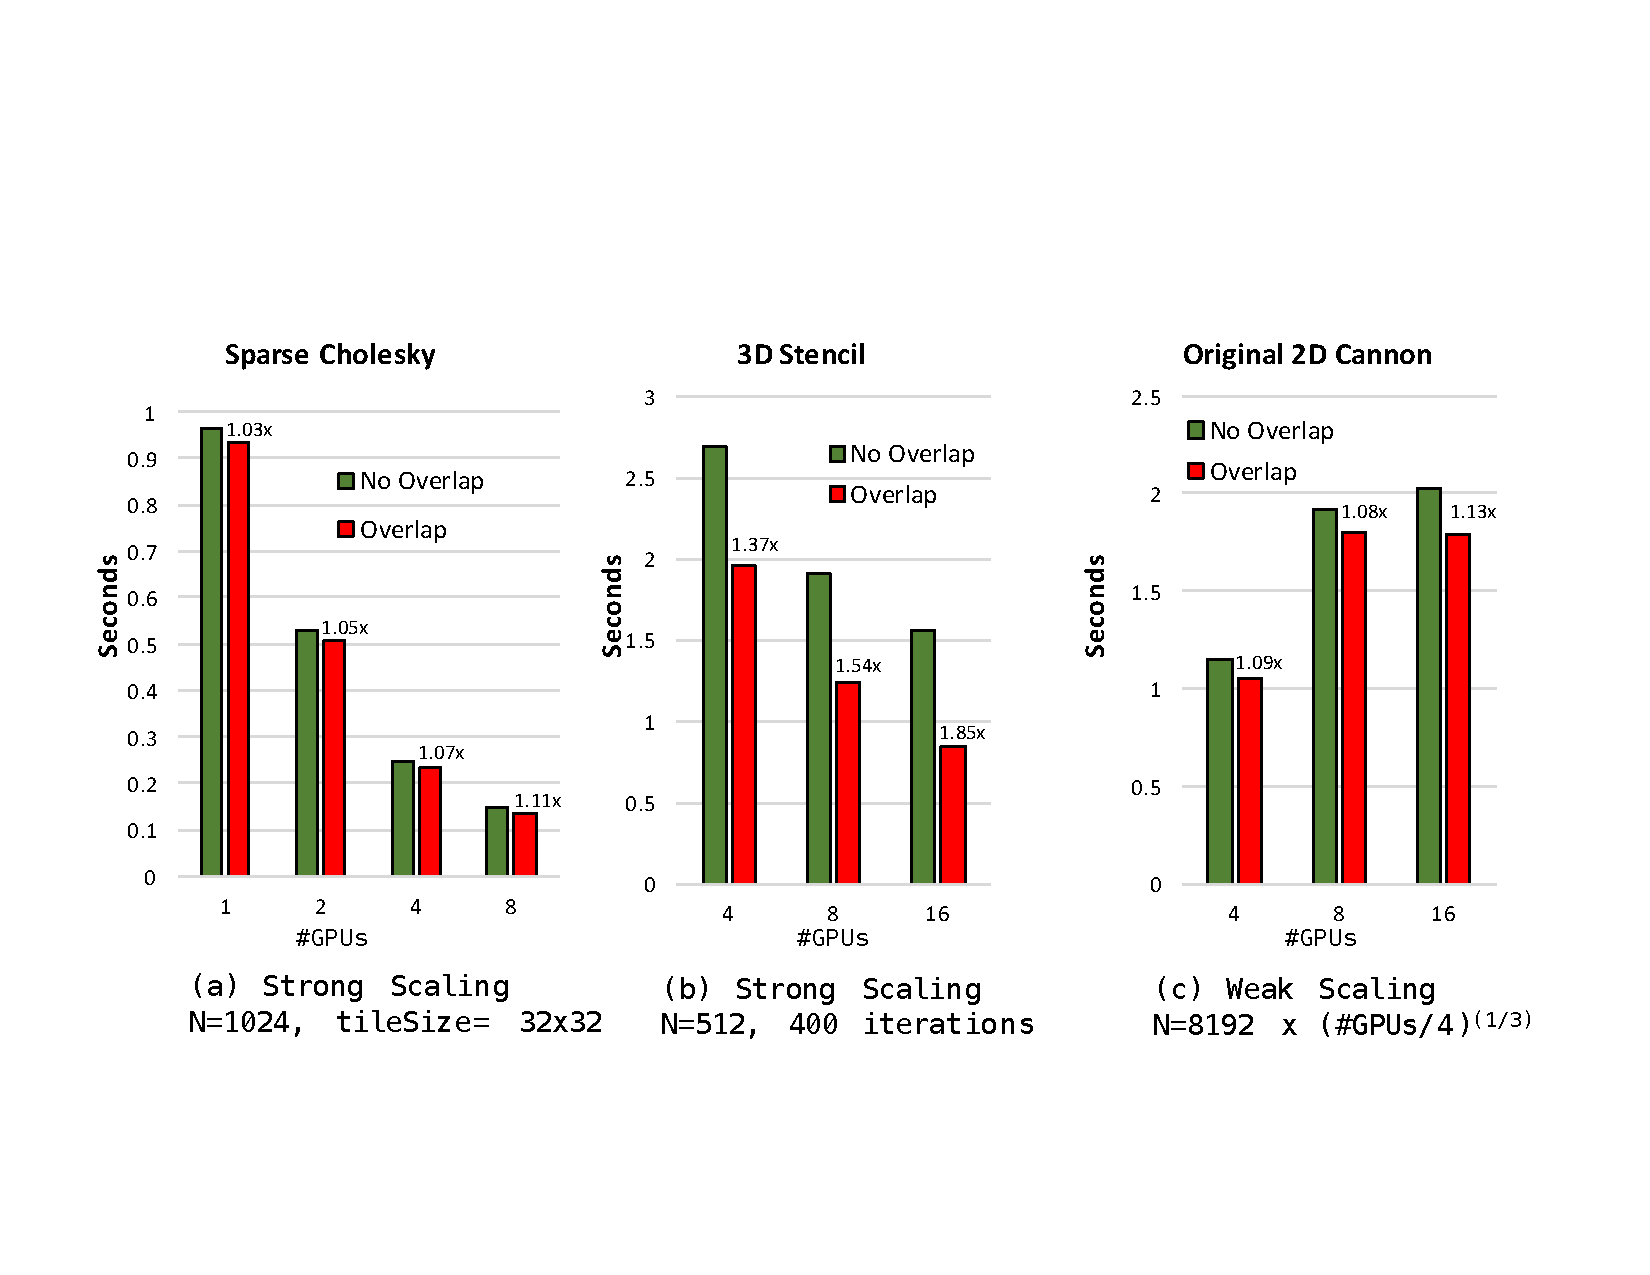
\includegraphics[width=0.9\textwidth]{figures/overlap.pdf}
\caption{Hiding communication automatically via overlap}
\label{overlap}
\end{figure*}

\begin{figure}[htb]
\centering
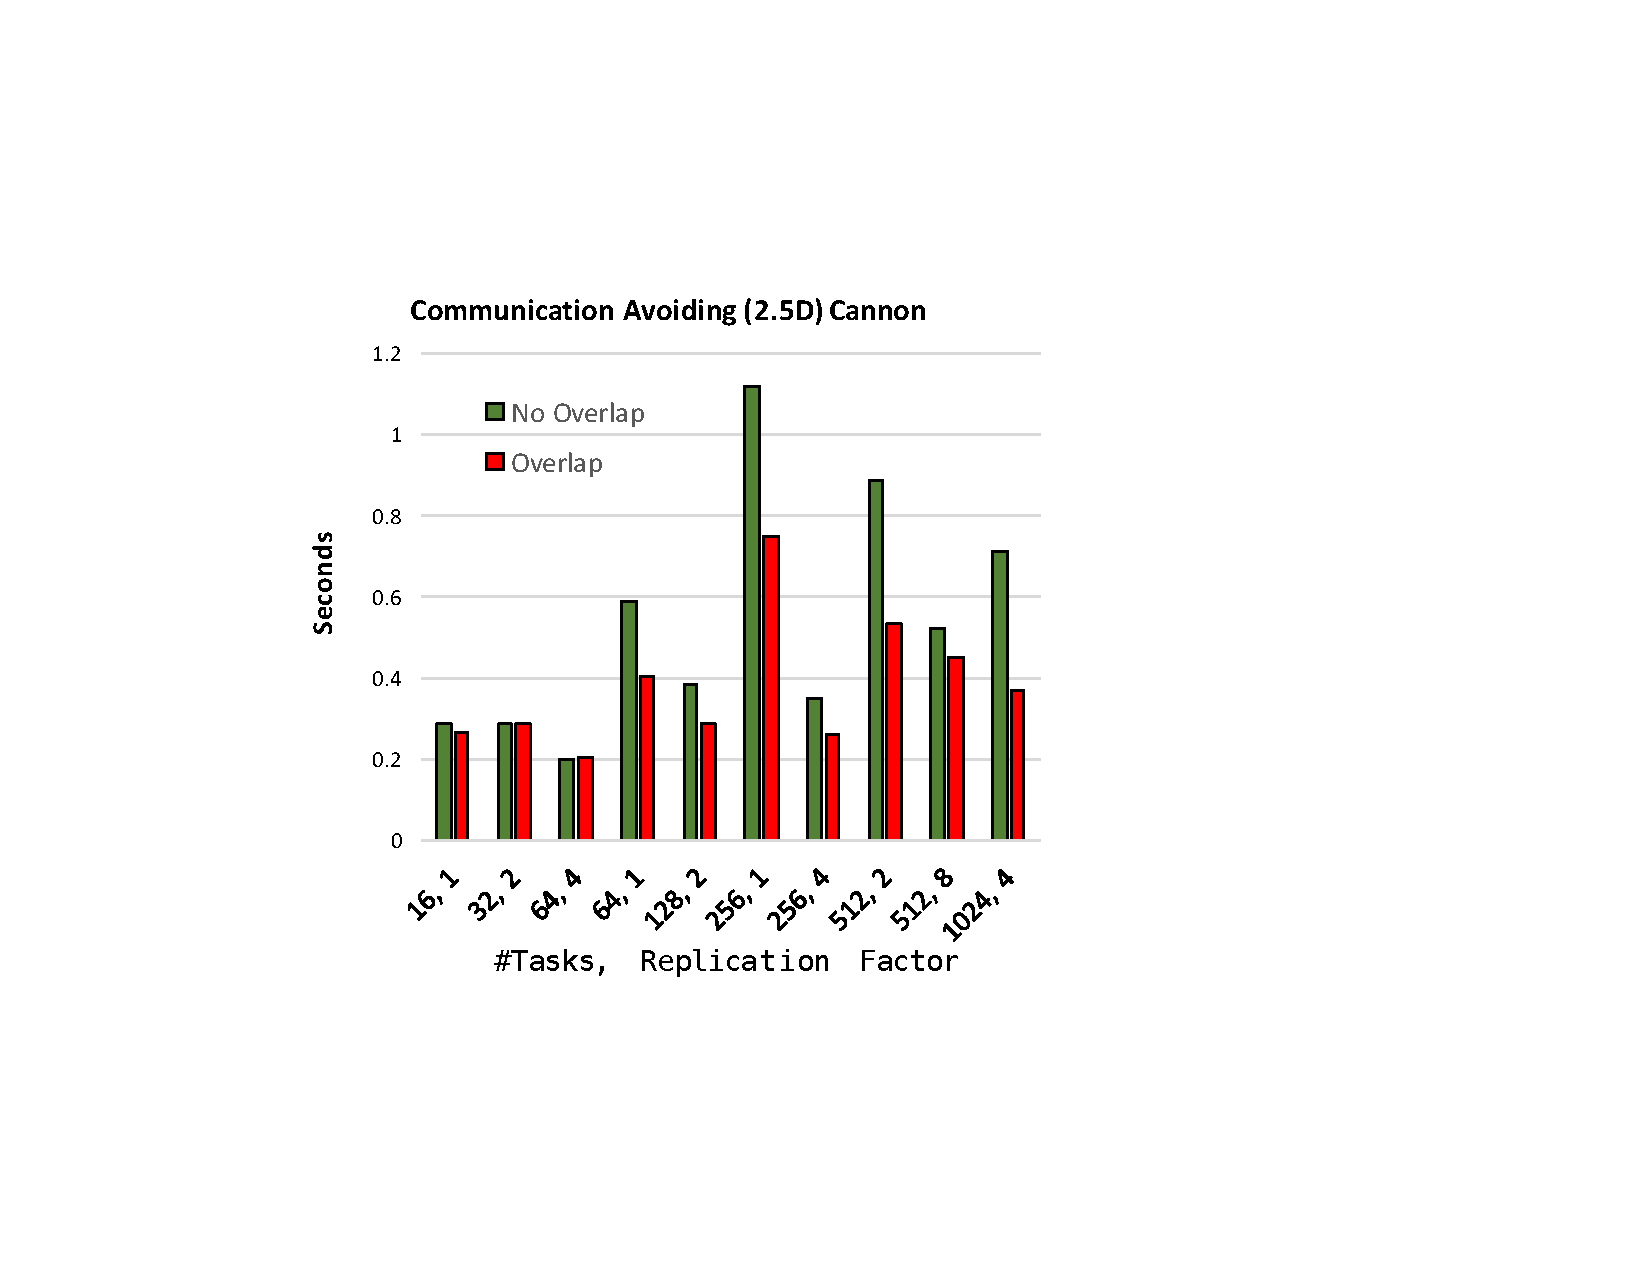
\includegraphics[width=0.49\textwidth]{figures/CA_4096.pdf}
\caption{2.5D Cannon on 16 GPUs using small matrices (N=4096). The communication avoiding technique results in many task configurations. For good configurations (e.g. \{64, 4\}), there is not much room for the communication overlap. However, for poor configurations (e.g. \{1024, 4\}) the overlap technique does a good job in further increasing the performance}
\label{CA_4096}
\end{figure}

\subsection{Interference between communication avoiding and hiding}
\label{subsec:CAvsOlap}
Now let's study the behavior of {\em overlap} when the communication avoiding technique is enabled.
Fig.~\ref{CA_4096} shows the run time of the 2.5D Cannon program when performing matrix multiplication on 16 GPUs.
We can see that replicating matrices substantially reduces the run time.
Notable examples are  \{64, 4\} compared to \{64, 1\} and \{256, 4\} compared to \{256, 1\}.
If most of the data communication can be avoided, there is not much left to hide.
However, the number of these optimal replication configurations is very small compared to the combination of task and replication spaces.
As a result, the programmer may need to brute force many potential configurations to find the best one.
This requirement is costly and time consuming.
Luckily the overlapping technique can work with communication avoiding within the same application.
Thus, if the programmer does not pick the best replication configuration, he/she can rely on the communication overlap to realize comparable performance.
For example, the {\em overlap} performance on configurations \{128, 2\}, \{256, 4\}, or the most wanted \{64, 1\} is  acceptable. 
We can see that there are many of such configurations, allowing the programmer to guess one easily.

